\documentclass{article}
\usepackage{verbatim}
\usepackage{hyperref}
\usepackage{tcolorbox}
\usepackage{booktabs}
\usepackage{siunitx}
\usepackage{threeparttable}
\usepackage{float}
\usepackage{graphicx}

\sisetup{
  detect-all,
  output-exponent-marker = \mathrm{e},
  table-number-alignment = center
}

\providecommand{\e}[1]{\ensuremath{\times 10^{#1}}}
\setlength{\parindent}{0pt}

\begin{document}

\title{Answers to Empirical IO I: Problem Set 1}
\author{}
\date{}
\maketitle

\begin{tcolorbox}
Q1. Look at the data and plot the distribution of distance to all schools, and the distribution of distance to the chosen school.
\end{tcolorbox}

\begin{figure}[H]
    \centering
    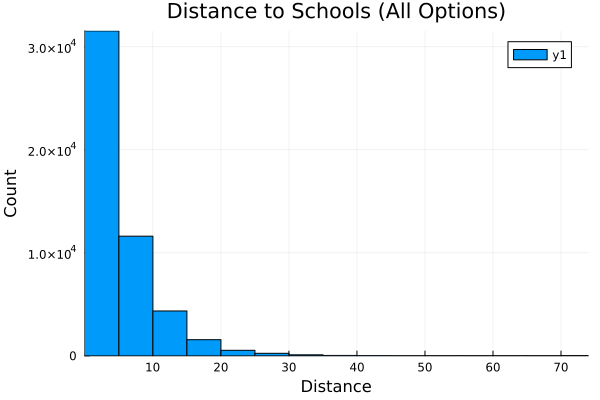
\includegraphics[width=0.5\textwidth]{outputs/Q1_dist_all.png}
    \caption{Distance to Schools (All Options)}
\end{figure}

\begin{figure}[H]
    \centering
    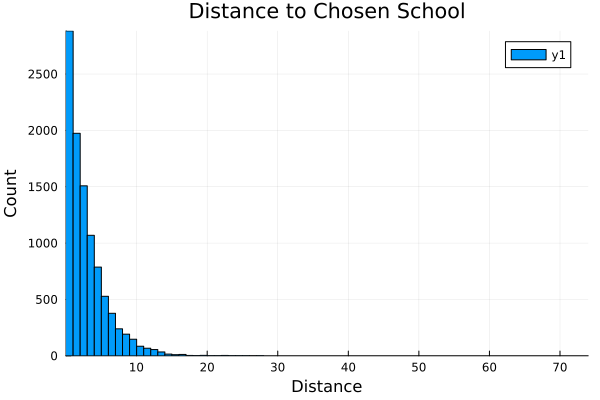
\includegraphics[width=0.5\textwidth]{outputs/Q1_dist_chosen.png}
    \caption{Distance to Chosen School}
\end{figure}

\vspace{5mm}

Clearly, chosen schools tend to be closer.
\begin{tcolorbox}
Q2. Write down the market share and log-likelihood for a plain logit model.
\end{tcolorbox}

Market share for a school $j$ comes from aggregating up the individual choice probabilities. The deterministic part of utility is:
\[
V_{ij} := \beta_1 \,\text{tests}_j + \beta_2 \,\text{sports}_j - \alpha \, d_{ij} + \xi_j
\]
The choice probability that household $i$ chooses school $j$ is
\[
P_{ij}(\theta) \;=\; \frac{\exp(V_{ij})}{\sum_{k=1}^J \exp(V_{ik})}.
\]
So the implied market share for school $j$ is jsut the average over all households:
\[
s_j(\theta) \;=\; \frac{1}{H} \sum_{i=1}^H P_{ij}(\theta).
\]

Let $y_{ij}\in\{0,1\}$ indicate whether household $i$ chose school $j$.
Given the choice probabilities above, the likelihood of the observed choice for household $i$ can be written as
\[
L_i(\theta) \;=\; \prod_{j=1}^J P_{ij}(\theta)^{\,y_{ij}}.
\]

With independence across households, the likelihood can be written out multiplicatively as:
\[
L(\theta) \;=\; \prod_{i=1}^H L_i(\theta) 
\;=\; \prod_{i=1}^H \prod_{j=1}^J P_{ij}(\theta)^{\,y_{ij}}.
\]
With the log-likelihood therefore simplifying to
\[
\ell(\theta) 
\;=\; \sum_{i=1}^H \sum_{j=1}^J y_{ij}\,\log P_{ij}(\theta).
\]




\begin{tcolorbox}
Q3. Write down the score and the gradient of your log-likelihood.
\end{tcolorbox}

The score and the gradient refer to the same thing: the first derivatives with respect to the model parameters (?)

\vspace{5mm}

Let $x_{ij} = \big(\text{tests}_j,\ \text{sports}_j,\ -d_{ij}\big)$. Using the log-likelihood above, the score is then
\[
\nabla_\theta \ell(\theta)
=
\left(
\sum_{i=1}^H \sum_{j=1}^J x_{ij}\,(y_{ij}-P_{ij}),
\;\;
\sum_{i=1}^H (y_{i1}-P_{i1}),
\ldots,
\sum_{i=1}^H (y_{iJ}-P_{iJ})
\right).
\]

Where the first block is a 3 dim vector of the derivatives wrt $(\beta_1,\beta_2,\alpha)$, and the remaining $J$ entries give the derivatives with respect to $(\xi_1,\ldots,\xi_J)$.

Or written out component-wise:
\[
\frac{\partial \ell}{\partial \beta_1}
=\sum_{i=1}^H\sum_{j=1}^J \text{tests}_j\,(y_{ij}-P_{ij}), 
\qquad
\frac{\partial \ell}{\partial \beta_2}
=\sum_{i=1}^H\sum_{j=1}^J \text{sports}_j\,(y_{ij}-P_{ij}),
\]
\[
\frac{\partial \ell}{\partial \alpha}
=\sum_{i=1}^H\sum_{j=1}^J (-d_{ij})\,(y_{ij}-P_{ij}),
\qquad
\frac{\partial \ell}{\partial \xi_j}
=\sum_{i=1}^H (y_{ij}-P_{ij}), \quad j=1,\ldots,J.
\]

\begin{tcolorbox}
Q4. Estimate the plain logit model by maximimum likelihood.
\end{tcolorbox}

\begin{table}[H]
\centering
\resizebox{\textwidth}{!}{%
\begin{tabular}{lcccccc}
\toprule
Model & NLL & $\beta_1$ & $\beta_2$ & $\alpha$ & $D_{12}$ & Avg. own dist. elas. \\
\midrule
Plain Logit & 12563.72 & -0.24 & 0.23 & 0.20 & 0.13 & -0.43 \\
\bottomrule
\end{tabular}
}
\caption{Estimation results for logit models.}
\end{table}


\begin{tcolorbox}
Q5. Estimate a restricted model with only $\xi_j$ parameters. Add that to your table.
\end{tcolorbox}

\begin{table}[H]
\centering
\resizebox{\textwidth}{!}{%
\begin{tabular}{lcccccc}
\toprule
Model & NLL & $\beta_1$ & $\beta_2$ & $\alpha$ & $D_{12}$ & Avg. own dist. elas. \\
\midrule
Plain Logit & 12563.72 & -0.24 & 0.23 & 0.20 & 0.13 & -0.43 \\\n$\text{Only-}\xi$ & 14260.39 & -- & -- & -- & -- & -- \\
\bottomrule
\end{tabular}
}
\caption{Estimation results for logit models.}
\end{table}

\begin{tcolorbox}
Q6. Now allow for parents to have different preferences for $\text{test scores}_j$ so that $\beta_{1i} \sim \mathcal{N}(\beta_1, \sigma_b)$. Write down the (simulated) market share and gradient expressions.
\end{tcolorbox}

Each household $i$ has a random coefficient $\beta_{1i}$ such that
\[
\beta_{1i} \sim \mathcal{N}(\beta_1,\sigma_b).
\]
The deterministic utility becomes
\[
V_{ij} = \beta_{1i}\,\text{tests}_j + \beta_2\,\text{sports}_j - \alpha\,d_{ij} + \xi_j.
\]

For a given household $i$ and a given draw $r$ from the normal, the choice probability is
\[
P_{ij}^{(r)}(\theta) \;=\; \frac{\exp\!\left(\beta_{1i}^{(r)}\,\text{tests}_j + \beta_2\,\text{sports}_j - \alpha\,d_{ij} + \xi_j\right)}
{\sum_{k=1}^J \exp\!\left(\beta_{1i}^{(r)}\,\text{tests}_k + \beta_2\,\text{sports}_k - \alpha\,d_{ik} + \xi_k\right)}.
\]

We can obtain the simulated market share by averaging over $R$ draws for each household:
\[
\tilde s_j(\theta) \;=\; \frac{1}{H}\sum_{i=1}^H \frac{1}{R} \sum_{r=1}^R P_{ij}^{(r)}(\theta).
\]

For the log-likelihood $\ell(\theta)=\sum_{i=1}^H\sum_{j=1}^J y_{ij}\log P_{ij}(\theta)$ with $P_{ij}$ replaced by its simulated counterpart, the (simulated) score components are obtained by averaging the per-draw contributions:
\[
\frac{\partial \ell}{\partial \beta_1}
=\sum_{i=1}^H \frac{1}{R}\sum_{r=1}^R 
\Big( \text{tests}_{j(i)} - \sum_{k=1}^J P_{ik}^{(r)}\,\text{tests}_k \Big),
\]
\[
\frac{\partial \ell}{\partial \beta_2}
=\sum_{i=1}^H \frac{1}{R}\sum_{r=1}^R 
\Big( \text{sports}_{j(i)} - \sum_{k=1}^J P_{ik}^{(r)}\,\text{sports}_k \Big),
\]
\[
\frac{\partial \ell}{\partial \alpha}
=\sum_{i=1}^H \frac{1}{R}\sum_{r=1}^R 
\Big( -d_{i\,j(i)} + \sum_{k=1}^J P_{ik}^{(r)}\,d_{ik} \Big),
\]
\[
\frac{\partial \ell}{\partial \xi_j}
=\sum_{i=1}^H \frac{1}{R}\sum_{r=1}^R \big( y_{ij} - P_{ij}^{(r)} \big), 
\qquad j=1,\ldots,J.
\]

There is also the additional parameter $\sigma_b$ governing the dispersion of of $\beta_{1i}$.

\[
\frac{\partial \ell}{\partial \sigma_b}
=\sum_{i=1}^H \frac{1}{R}\sum_{r=1}^R 
z_{ir}\,\Big( \text{tests}_{j(i)} - \sum_{k=1}^J P_{ik}^{(r)}\,\text{tests}_k \Big),
\]

Because $\beta_{1i}^{(r)} = \beta_1 + \sigma_b z_{ir}$, the chain rule gives 
$\partial \beta_{1i}^{(r)} / \partial \sigma_b = z_{ir}$, which is why a factor $z_{ir}$ multiplies the same test-score score component as for $\beta_1$.



\begin{tcolorbox}
Q7. Estimate this expanded model via maximum likelihood: (a) Using 100 Monte Carlo Draws from an appropriately transformed standard normal. (b) Using a Gauss Hermite quadrature rule.
\end{tcolorbox}

\begin{table}[H]
\centering
\resizebox{\textwidth}{!}{%
\begin{tabular}{lcccccc}
\toprule
Model & NLL & $\beta_1$ & $\beta_2$ & $\alpha$ & $D_{12}$ & Avg. own dist. elas. \\
\midrule
Plain Logit & 12563.72 & -0.24 & 0.23 & 0.20 & 0.13 & -0.43 \\\n$\text{Only-}\xi$ & 14260.39 & -- & -- & -- & -- & -- \\\n Expanded Logit (MC, R=100) & 12563.72 & -0.17 & 0.25 & 0.20 & 0.13 & -0.43 \\\n Expanded Logit (GH, M=20) & 12563.72 & -0.17 & 0.25 & 0.20 & 0.13 & -0.43 \\
\bottomrule
\end{tabular}
}
\caption{Estimation results for logit models.}
\end{table}


\begin{tcolorbox}
Q8. Read Chapter 10 in Train and write down the MSM estimator for the expanded model. What are your ``instruments''?
\end{tcolorbox}

The MSM estimator takes the residuals from the simulated model of choice probabilities and projects them onto a set of (exogenous) variables. Specifically, for each household $i$ and school $j$ we observe $y_{ij}\in\{0,1\}$, and we compute simulated probabilities $\hat P_{ij}(\theta)$ given parameters $\theta=(\beta_1,\beta_2,\alpha,\sigma_b,\xi)$.  

\vspace{5mm}

To construct the MSM estimator, we take the simulated residuals 
\[
y_{ij} - \hat P_{ij}(\theta)
\]
and require that, on average, they are uncorrelated with the chosen instruments $z_{ij}$.  
Formally, this means imposing the moment conditions
\[
\frac{1}{H}\sum_{i=1}^H \sum_{j=1}^J 
\bigl(y_{ij} - \hat P_{ij}(\theta)\bigr)\, z_{ij} \;=\; 0.
\]
Since in practice the sample moments will not be exactly zero, the MSM estimator chooses $\theta$ to make them as close to zero as possible.  
That is,
\[
\hat{\theta}_{MSM}
= \arg\min_{\theta}\;
\left\|
\frac{1}{H}\sum_{i=1}^H \sum_{j=1}^J 
\bigl(y_{ij} - \hat P_{ij}(\theta)\bigr)\, z_{ij}
\right\|^2,
\]
where the norm reflects the weighting we put on different instruments.


\medskip
\noindent
The instruments $z_{ij}$ are variables that shift the observed choices but are not correlated with the unobserved school quality terms $\xi_j$.  
We might plausibly just use our observables to instrument themselves, given they are not part of $\xi_j$) and they correlate strongly with the residuals $(y_{ij}-\hat P_{ij}(\theta))$.

\vspace{5mm}

So in practice, the MSM estimator here would be computed by driving the average residuals interacted with distance, tests, and sports to zero.  


\begin{tcolorbox}
Q9. Calculate the Jacobian of the MSM estimator.
\end{tcolorbox}

As above, we have the moment conditions:
\[
g_H(\theta) \;=\; \frac{1}{H}\sum_{i=1}^H \sum_{j=1}^J 
\bigl(y_{ij}-\hat P_{ij}(\theta)\bigr)\, z_{ij}.
\]

The Jacobian is the matrix of first derivatives, which we can calculate by the chain rule:
\[
G(\theta)\;:=\;\frac{\partial g_H(\theta)}{\partial \theta^\top}
\;=\;-\frac{1}{H}\sum_{i=1}^H\sum_{j=1}^J z_{ij}\,\Bigl(\frac{\partial \hat P_{ij}(\theta)}{\partial \theta^\top}\Bigr).
\]

$\hat P_{ij}(\theta)$ is a simulation (I'll use GH) average over draws $r=1,\ldots,R$:
\[
\hat P_{ij}(\theta)\;=\;\frac{1}{R}\sum_{r=1}^R P^{(r)}_{ij}(\theta),\qquad
P^{(r)}_{ij}=\frac{\exp(V^{(r)}_{ij})}{\sum_{k=1}^J \exp(V^{(r)}_{ik})},
\]
so
\[
\frac{\partial \hat P_{ij}}{\partial \theta}
\;=\;\frac{1}{R}\sum_{r=1}^R \frac{\partial P^{(r)}_{ij}}{\partial \theta}.
\]

For the logit probability
\[
P^{(r)}_{ij}(\theta)
= \frac{\exp(V^{(r)}_{ij})}{\sum_{k=1}^J \exp(V^{(r)}_{ik})},
\]
the derivative with respect to a parameter $\theta$ is
\[
\frac{\partial P^{(r)}_{ij}}{\partial \theta}
= P^{(r)}_{ij}\Bigl(x^{(r)}_{ij,\theta}
- \sum_{k=1}^J P^{(r)}_{ik}\,x^{(r)}_{ik,\theta}\Bigr),
\]
where $x^{(r)}_{ij,\theta} := \partial V^{(r)}_{ij}/\partial\theta$.

\vspace{5mm}

In our model 
\[
V^{(r)}_{ij}
= \beta_{1i}^{(r)}\,\text{tests}_j
+ \beta_2\,\text{sports}_j
- \alpha\,d_{ij}
+ \xi_j,
\qquad
\beta_{1i}^{(r)}=\beta_1+\sigma_b z_{ir}.
\]
Hence the relevant derivatives are
\[
x^{(r)}_{ij,\beta_1}=\text{tests}_j,\qquad
x^{(r)}_{ij,\sigma_b}=z_{ir}\,\text{tests}_j,\qquad
x^{(r)}_{ij,\beta_2}=\text{sports}_j,\qquad
x^{(r)}_{ij,\alpha}=-d_{ij},\qquad
x^{(r)}_{ij,\xi_m}=\mathbb{1}\{j=m\}.
\]

Substituting these into the expression above gives the derivatives of the probabilities with respect to each parameter, which are then used in the Jacobian $G(\theta)$.

\begin{tcolorbox}
Q10. Estimate the Parameters of the MSM estimator.
\end{tcolorbox}

\begin{table}[H]
\centering
\resizebox{\textwidth}{!}{%
\begin{tabular}{lcccccc}
\toprule
Model & NLL & $\beta_1$ & $\beta_2$ & $\alpha$ & $D_{12}$ & Avg. own dist. elas. \\
\midrule
Plain Logit & 12563.72 & -0.24 & 0.23 & 0.20 & 0.13 & -0.43 \\\n$\text{Only-}\xi$ & 14260.39 & -- & -- & -- & -- & -- \\\n Expanded Logit (MC, R=100) & 12563.72 & -0.17 & 0.25 & 0.20 & 0.13 & -0.43 \\\n Expanded Logit (GH, M=20) & 12563.72 & -0.17 & 0.25 & 0.20 & 0.13 & -0.43 \\\n MSM (GH, M=20) & -- & -0.13 & 0.24 & 0.20 & 0.16 & -0.43 \\
\bottomrule
\end{tabular}
}
\caption{Estimation results for logit models.}
\end{table}

\begin{tcolorbox}
Q11. Bonus: Using your initial MSM estimates as a starting point, explain how to construct an ``efficient'' MSM estimator, and produce ``efficient'' estimates.
\end{tcolorbox}

Efficiency comes from using the right weighting matrix $W$ on the moment conditions. We can construct the efficient MSM by:

\textbf{Step 1 (initial):} estimate $\hat\theta^{(1)}$ with one–step MSM using $W=I$, as in the last question. 
This gives us consistent but not necessarily efficient estimates, since it treats each moment condition as equally informative.

\vspace{5mm}

\textbf{Step 2 (weighting):} at $\hat\theta^{(1)}$, form per-household moment vectors
\[
m_i(\theta)=\sum_{j=1}^J \big(y_{ij}-\hat P_{ij}(\theta)\big)\,z_{ij},
\qquad
g_H(\theta)=\frac{1}{H}\sum_{i=1}^H m_i(\theta).
\]
Here $m_i(\theta)$ measures the discrepancy between observed choices and predicted probabilities, weighted by the instruments $z_{ij}$. 
The covariance of these discrepancies tells us which moments are measured more precisely. 
Following Train Chapter 10, we can estimate this covariance as
\[
\widehat S=\frac{1}{H}\sum_{i=1}^H\Big(m_i(\hat\theta^{(1)})-g_H(\hat\theta^{(1)})\Big)
\Big(m_i(\hat\theta^{(1)})-g_H(\hat\theta^{(1)})\Big)^\top,
\]
and set $W=\widehat S^{-1}$ to give higher weight to the more informative moments.

\vspace{5mm}

\textbf{Step 3 (re-estimate):} solve
\[
\hat\theta^{(2)}=\arg\min_\theta g_H(\theta)^\top W\, g_H(\theta).
\]
This re-estimation with the optimal weight matrix yields the efficient MSM estimator. See estimates in cumulative trade table below:

\begin{table}[H]
\centering
\resizebox{\textwidth}{!}{%
\begin{tabular}{lcccccc}
\toprule
Model & NLL & $\beta_1$ & $\beta_2$ & $\alpha$ & $D_{12}$ & Avg. own dist. elas. \\
\midrule
Plain Logit & 12563.72 & -0.24 & 0.23 & 0.20 & 0.13 & -0.43 \\\n$\text{Only-}\xi$ & 14260.39 & -- & -- & -- & -- & -- \\\n Expanded Logit (MC, R=100) & 12563.72 & -0.17 & 0.25 & 0.20 & 0.13 & -0.43 \\\n Expanded Logit (GH, M=20) & 12563.72 & -0.17 & 0.25 & 0.20 & 0.13 & -0.43 \\\n MSM (GH, M=20) & -- & -0.13 & 0.24 & 0.20 & 0.16 & -0.43 \\\n Efficient MSM (GH, M=20)) & -- & -0.13 & 0.24 & 0.20 & 0.16 & -0.43 \\
\bottomrule
\end{tabular}
}
\caption{Estimation results for logit models.}
\end{table}


\end{document}
